\chapter{Situation}



\section{Scenario Overview}



\begin{rpg-commentbox}{Overview}
    ``\textit{Be a real shame if the lowest bidder on that fire safety system cut corners to increase their profit margin.}''

    \begin{flushright}
    -- Joker4-1
    \end{flushright}

    A space shuttle ambulance brings a high-priority patient to San Cristobal Medical Facility. The shuttle belongs to Weyland-Yutani crew and they had pulled strings to avoid any security clearances or quarantine measures expected by normal crew. Whoever or whatever they bring is high enough in the food chain that the facility makes room for them. It is not like shift workers who suffered any accidents need a hospital bed.
    
    The patient has a xenomorph embryo growing inside them and  Weyland-Yutani is eager to extract the asset. This would have been a profitable day for the corporation if not by a second xenomorph who has lurked in the shuttle waiting for an easy prey. As the shuttle lifts, the alien strikes embracing the pilot---in the now pressurized cabin---to their death. Adrift, the shuttle violently clashes in the landing area causing a
    huge blast that propagates through the facility.
\end{rpg-commentbox}


\begin{rpg-commentbox}{Fire Brigade}
    Players are firefighters that now need to assess the situation and suppress 
    the raging fire before the station's computer---APOLLO---decides that the area is too hazardous and that it should be detached from the main structure before it compromises the entire station.

    There are many things at stake, such as the lives of skilled crew, 
    scientific data from assorted companies and billions of dollars in company assets. As a firefighter, this is the worst imaginable situation, and some of 
    you know that sacrifices will be made.
\end{rpg-commentbox}


\newsect

\begin{rpg-commentbox}{Before the firefighters arrival}
    Living in space is hell and everyone knows that. Most of the staff that could have escaped tha facility has already left, carrying low-risk patients that could have held their own with them. 

    Unfortunately, security measures from the facility also took place sealing doors in hope that the fire suppression system can minimize the fire/damage. 
    This has made several sections of the facility inaccessible and only skilled firefighters can make their way throughout the chaos.
\end{rpg-commentbox}


\newsect


\begin{figure}[!b]
    \centering
    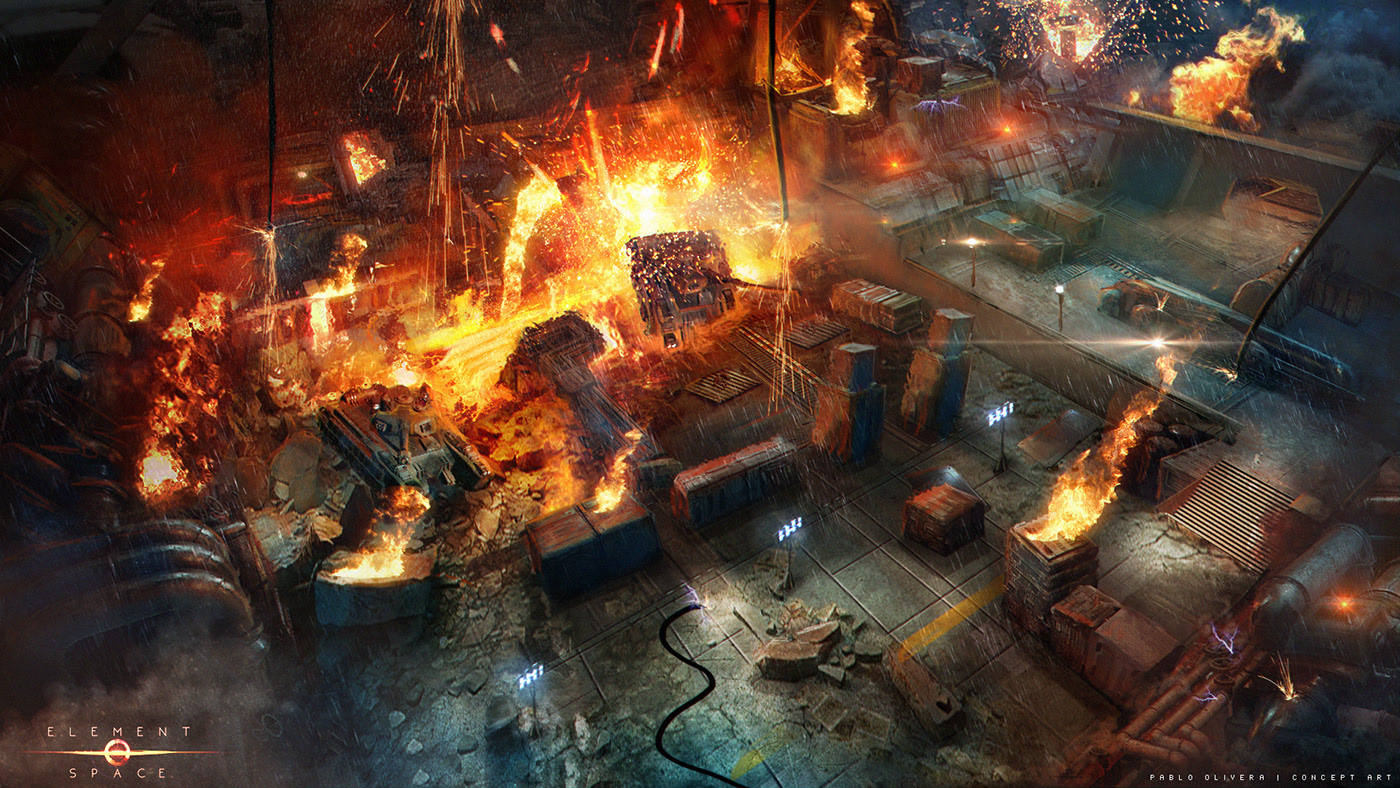
\includegraphics[width=.45\textwidth]{img/bg/fire.jpg}
\end{figure}


\clearpage



\medskip
\begin{rpg-commentbox}{Firefighting in Space}
\begin{small}
    \textit{Firefighters usually only enter a building when it is safe enough to do so. Their priority is to search for survivors, find the source of the fire so they can assess how to better suppress it as well as find any power or electrical sources that must be disabled so that they can act as best as they can.}

    \textit{Visibility is one of the major problems while sweeping a building. For the purposes of the game, it is an impeding factor, but one that is not as accurate as it should be. Due to smoke, firefighters usually crouch and stay as close to the floor as they can. This is also to sweep the floor in front of them, find any victims, and avoid stumbling over any dangers.}

    \textit{There is a lot of cordination among firefighters and a ``chief'' assess everything from a safe place where he can call the shots and request firefighters to evacuate before they are trapped in the fire themselves, give priority to a more important matter, etc.}

    \textit{A potential complication on using water to suppress fires in a space station is that it can cause more electrical fires, or damage corporate equipment. For small electrical panels, fire extinguishers are a common tool.For bigger areas engulfed by the fire, standard procedures are to seal blocks of a building and vent all the air away, or to pray that the gaseous fire suppression systems have done their job. }

    \textit{Accidentally sucking all the air from a building is also not something that should be easily accessible---you don't want a toddler pulling a lever and killing dozens of people. Hence, these security measures are placed under well sealed hatches that can be pried open by a ``haligan'' tool or a welding torch.  }

    \textit{Sealing all doors before pulling the vent mechanism in large rooms is extremely problematic and this might force space firefighters to split up so that they can cover such large rooms. For example, in a T shape corridor, one firefighter stays near the entrance while the other rushes, closes the middle door and makes his way to the other side. As time is valuable, the firefighter proceeds to the next room, closes the door behind them and as soon as that is done, the firefighter who stayed behind pulls the lever venting all air out of that section. Once it is safe to proceed, they will meet the firefighter in the next room who is already taking similar measures.}

    \textit{What about victims? Crew might be expandable and corporate assets are often a priority. Standard procedure is to assess a victim's patch and check their role. Scientists or high corporate staff are too valuable and whenever possible, should be rescued. Unfortunately, the same is not true for roughnecks or security personnel. This puts firefighters in an odd position in a space station, some have made personal connections or even relationships that often clash with their role. Notably, roughnecks appreciate the job of  firefighters when it's just an everyday heavy machinery accident but they loathe them in the aftermath of a fire. Although rotating through stations so that any griefs between crew and firefighters can heal is not uncommon, sometimes this is not possible and firefighters face several mental health problems.}

\end{small}
\end{rpg-commentbox}


\newsect

\medskip


\medskip
\begin{rpg-commentbox}{Fire Supression}
\begin{small}
    \textit{Gaseous fire suppression, also called clean agent fire suppression, is a term to describe the use of inert gases and chemical agents to extinguish a fire.}    

    \textit{Systems working on a total flooding principle apply an extinguishing agent to a three dimensional enclosed space in order to achieve a concentration of the agent (volume percent of the agent in air) adequate to extinguish the fire. These types of systems may be operated automatically by detection and related controls or manually by the operation of a system actuator.}

\end{small}
\end{rpg-commentbox}

\newsect


\medskip
\begin{rpg-commentbox}{Halon}
\begin{small}
    \textit{Halon is a liquefied, compressed gas that stops the spread of fire by chemically disrupting combustion.}

    \textit{Halon leaves no residue and doesn't generally destroy sensitive items like paper and electronics, unlike foam, water, CO2, dry chem, etc. It's a nice perk to be able to suppress fire in a data center without having to write off ten million dollars worth of server equipment because it was destroyed by whatever you used to put out the fire.}

    \textit{While the two currently used types of halon gas are not generally considered deadly, they can still produce toxic by-products as they work to extinguish a fire.}

    \textit{High concentrations of halon can create an oxygen-deficient environment. This can cause people to suffocate.}
\end{small}
\end{rpg-commentbox}


\clearpage


\begin{rpg-commentbox}{Mainframes and Synthetics}
\begin{small}
    \textit{Synthetics do not breath and do not suffer from stress. One would expect that they would be used for such hazardous endeavor. 
    However, they are \textbf{expensive} and not easily replaceable, so only defective synthetics are ever provided to a fire station. }


    \textit{The rudimentary working Joes 
    sold by Seegson Corporation are also not a viable alternative. Their motor system is lack lusting making them move at a slow pace, and their neural synapses do not respond well to complex situations. Usually working Joes just drag victims out of a building whenever a fire alarm rings. Seegson Corporation answers to several law suits from people trying to get disability benefits after a working Joe dragged them to safety.}

    \textit{When a fire does not damage the structural integrity of a building, MU/TH/UR or APOLLO often perform venting supression procedures automatically. In case of damages, the system provides security footage that a fire marshall can use for tactical assessment. Nonetheless, security footage is often not available because this can be used for liability. Insurance companies often seek footage and sometimes even install rogue monitoring systems so they do not pay exorbitant values in the ever moving corporate chess.}

\end{small}
\end{rpg-commentbox}

\newsect



\medskip
\begin{rpg-commentbox}{Setting game difficulty}
\begin{itemize}
    \item \textbf{Normal}: as described in the booklet;
    \item \textbf{Hard}: firefighters are \textbf{sleep deprived}; 
    
    The last 24h shift was a living hell and firefighters really don't know how people stay alive in this shitty station---built with second-hand and cheap equipment. 
    
    This is similar to the \textit{exhaustion} game mechanics,
    but \texttt{\textbf{STAMINA}} rolls are called at the DM discretion such as when you are hiding from an alien and trying to stay awake at the same time. 
    
    Good luck with that ;)
\end{itemize}
\end{rpg-commentbox}




\begin{figure}
    \centering
    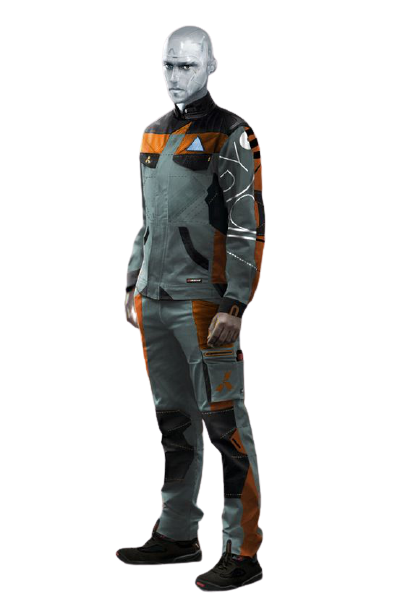
\includegraphics[width=.55\textwidth]{img/bg/working-joe.png}
    \label{fig:refinery}
\end{figure}

\clearpage


\begin{figure*}
    \centering
    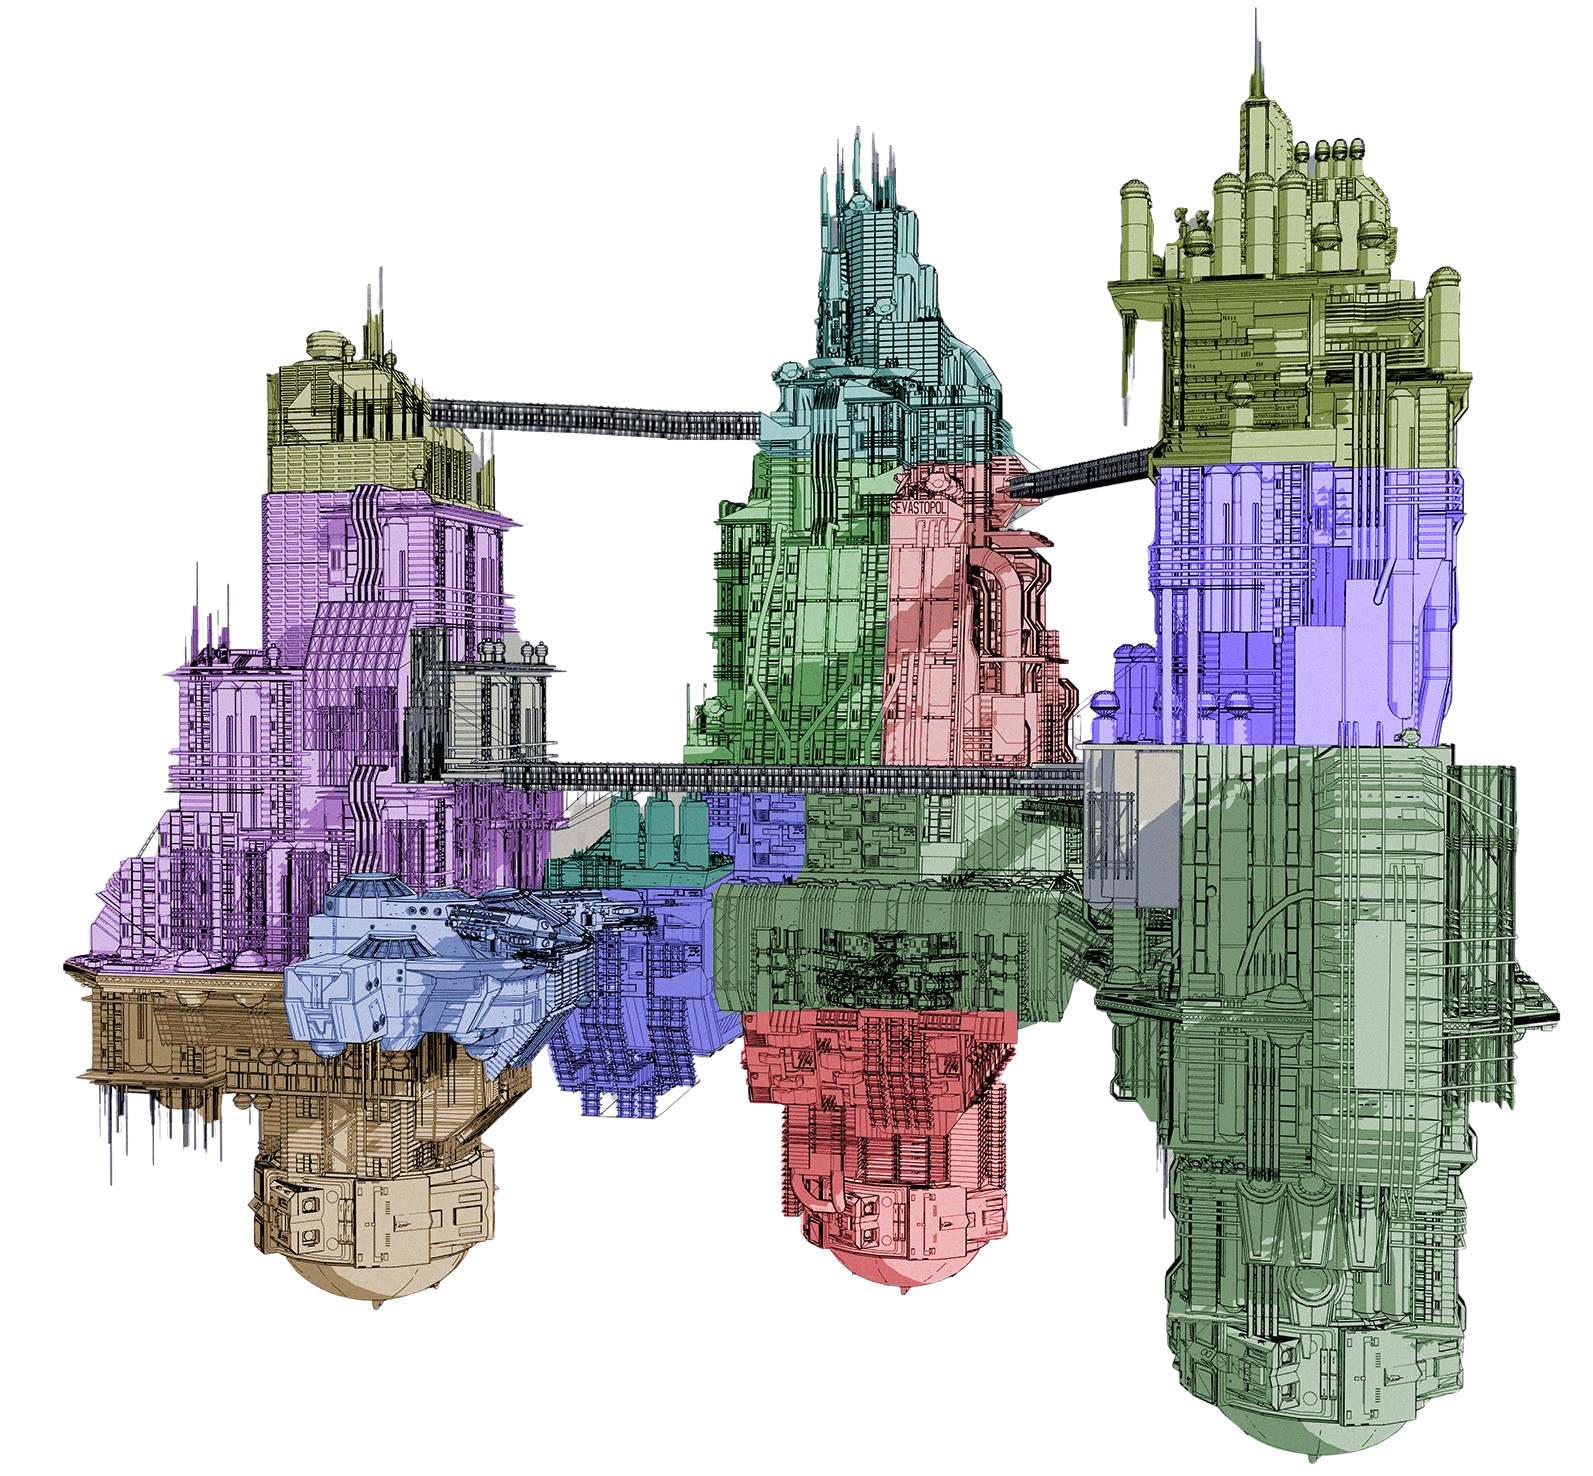
\includegraphics[width=1.0\textwidth]{img/bg/station.png}
\end{figure*}



% \makebox[0pt][l]{%
%   \raisebox{-\totalheight}[0pt][0pt]{%
%     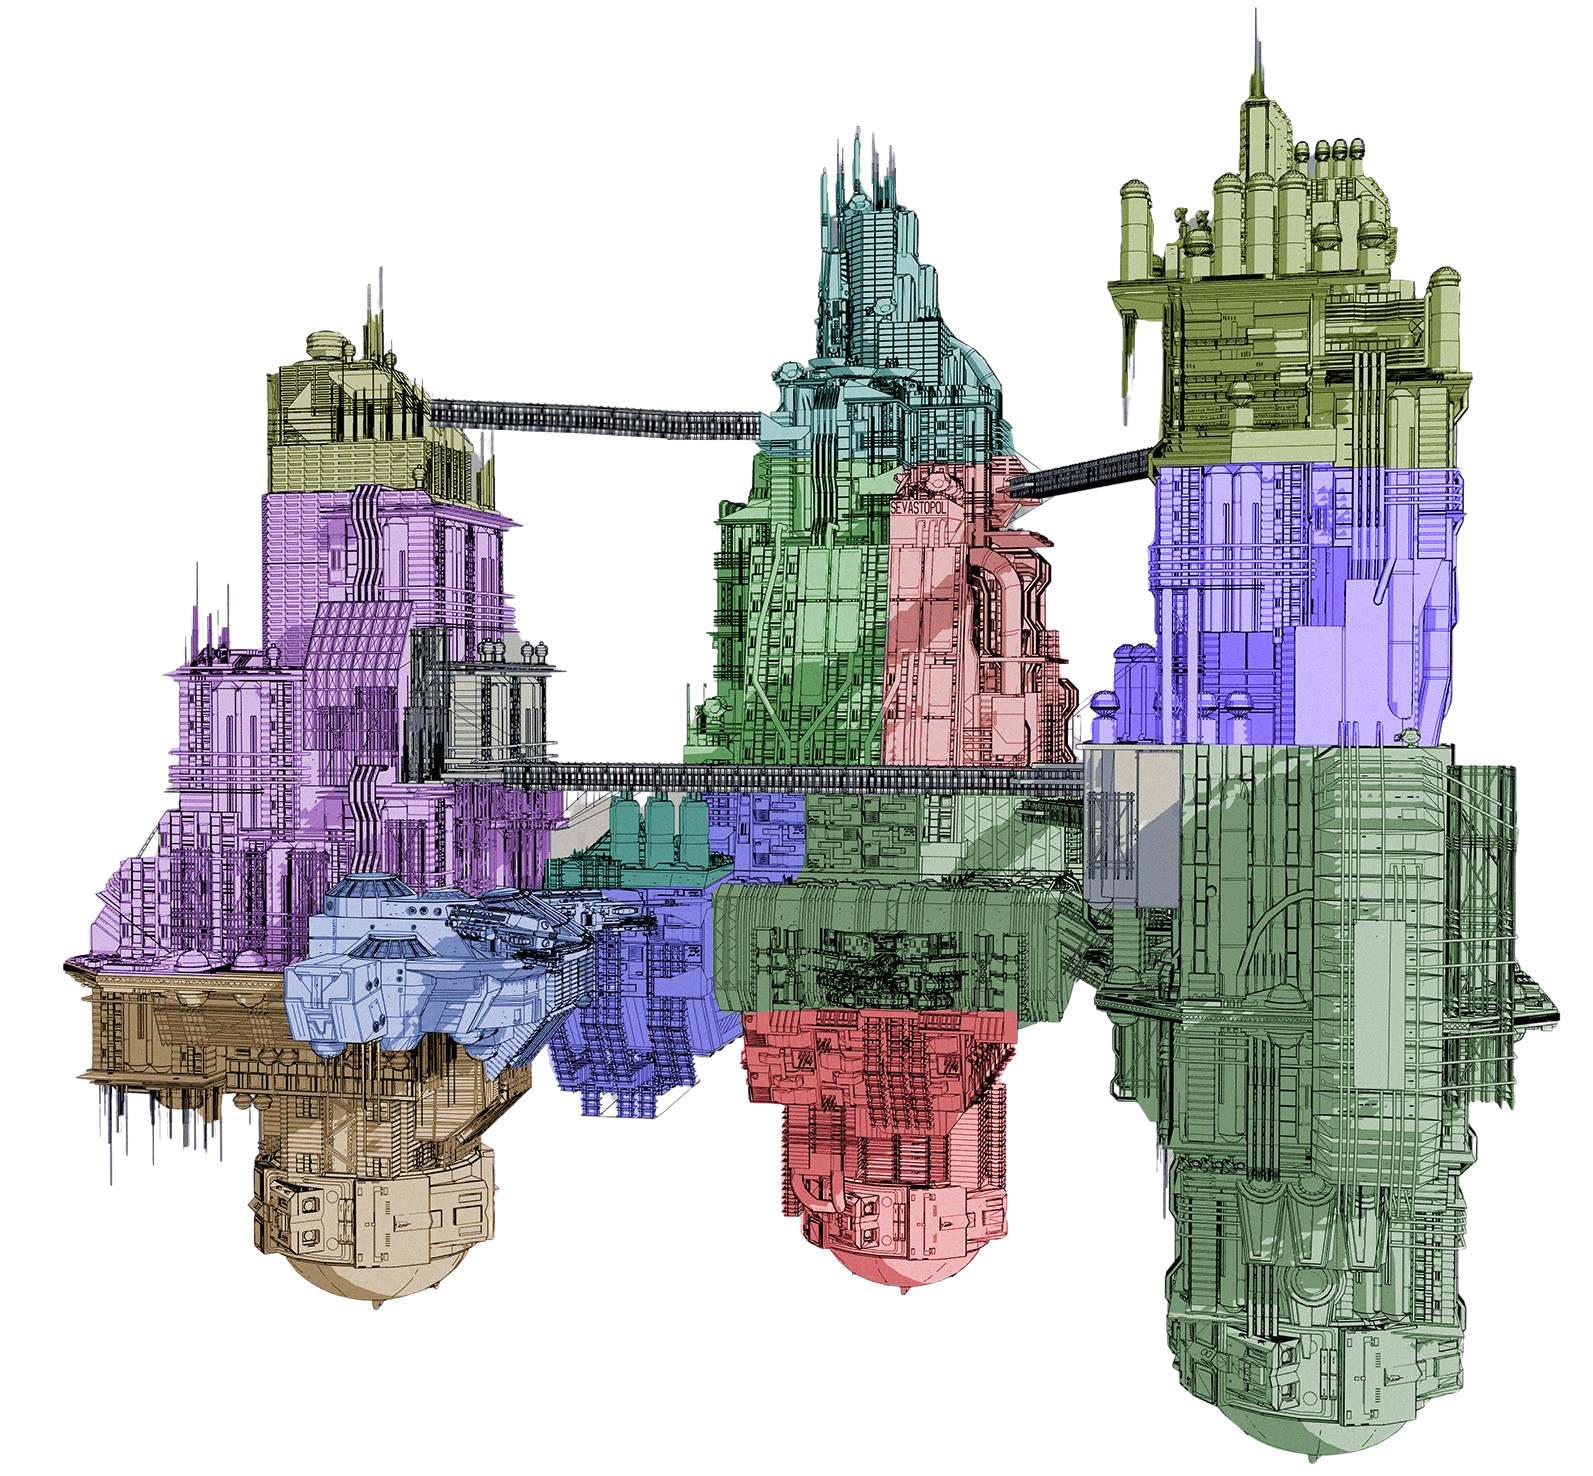
\includegraphics[width=1.30\textwidth]{img/bg/station.png}}}%









% \begin{figure*}
%     \centering
%     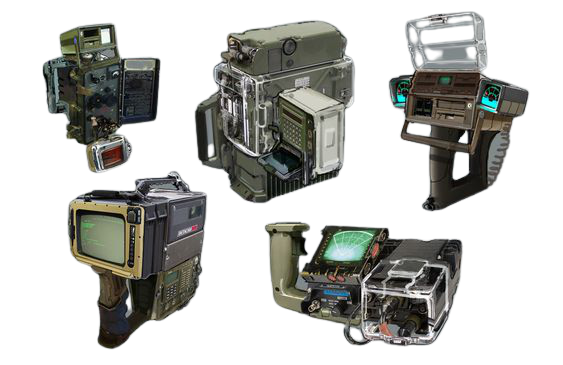
\includegraphics[width=1.0\textwidth]{img/bg/motion-tracker.png}
% \end{figure*}

% \newpage

% \begin{figure*}
%     \centering
%     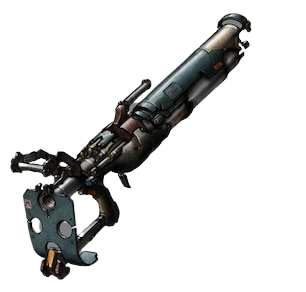
\includegraphics[width=1.0\textwidth]{img/bg/torch.png}
%     \label{fig:refinery}
% \end{figure*}

% \newpage

% \begin{figure*}
%     \centering
%     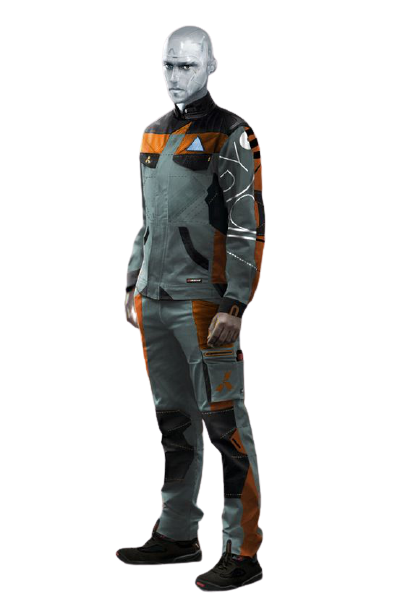
\includegraphics[width=1.0\textwidth]{img/bg/working-joe.png}
%     \label{fig:refinery}
% \end{figure*}
